\section{Caracterização das chuvas intensas}

A intensidade máxima média de precipitação cresce à medida que aumenta o período de retorno, sendo diretamente proporcionais, e decresce com o aumento da duração do evento, sendo inversamente proporcional a duração \cite{analise-chuva}. A principal forma de caracterização de chuvas intensas é por intermédio das equações de intensidade, duração e frequência da precipitação pluvial (equações IDF), ou equações de chuvas intensas \cite{tucci1993}, mais comumente representadas na forma da Equação \ref{eq:equacao-geral}. Estas equações são uma das ferramentas mais utilizadas nos trabalhos de engenharia relacionadas a recursos hídricos \cite{desagregacao}.

\begin{equation}
\label{eq:equacao-geral}
    i = \frac{k \times T_r^a}{(t+b)^c}
\end{equation}

Em que:

i = Intensidade máxima média de precipitação  $[mm.h^-1]$ 

$T_r$ = Período de retorno [anos]

t = Duração [min]

K, a, b, c = Parâmetros de ajuste estatístico, referentes à cada localidade

Para cada localidade ou plataforma de coleta de dados é feito, individualmente, o ajuste da equação para chuvas intensas. Recomenda-se ser feito com a utilização de um extenso período de dados, constituída de pluviógrafos \cite{interpolacao-chuva} apropriado a cada precipitação específica ocorrida em um posto pluviométrico, durante anos de observação. Entretanto, tais pluviógrafos dificilmente são disponíveis em quantidade e qualidade apropriada, devido à baixa densidade de equipamentos registradores espalhados no país, e às séries disponíveis serem frequentemente curtas e com falhas nos registros \cite{relacao-precipitacao}.

O estabelecimento de cada equação utiliza metodologia de exaustivo trabalho de tabulação, análise e interpretação de grande quantidade de pluviogramas, fitas utilizadas no registro por pluviógrafos \cite{relacao-precipitacao}. 

Decorrente da dificuldade de obtenção dos dados pluviográficos, a grande parte dos estudos realizados no Brasil, são efetuados com séries históricas inferiores à recomendada \cite{variabilidade-espacial}. A Organização Mundial de Meteorologia (OMM) recomenda a adoção de série histórica de no mínimo 30 anos.

Na prática, é difícil fixar o valor de intensidade da chuva, uma vez que o impacto é variável de local para local, seja em área rural ou urbana \cite{hidro-basica}. Em países subdesenvolvidos, as redes de dados climatológicos existentes são esparsas e escassas, reflexo na má qualidade dos projetos, originando obras sub ou superestimadas, quando superestimadas, podem gerar um desperdício econômico; e quando subestimadas, uma redução da confiabilidade de eficiência da obra e aumento do risco \cite{tucci1993}. Por esta razão, há barreiras na realização de projetos de obras hidráulicas mais confiáveis e econômicos \cite{chuva-bahia}. 

A busca por uma associação intensidade-duração-frequência de uma chuva é anterior a 1932 \cite{desagregacao}. Desde 1960 países desenvolvidos tem estudado a sua distribuição geográfica, onde possuem mapas que fornecem as intensidades e alturas de precipitação \cite{desagregacao}. Os estudos pioneiros no Brasil foram desenvolvidos por Pfafstetter (1957) e Denardin e Freitas (1982), em que Denardin e Freitas (1982) ajustaram equações matemáticas, a partir de gráficos apresentados por Pfafstetter (1957), que possibilitaram cálculo das alturas pluviométricas, em função da duração da precipitação e do período de retorno, por meio do método de regressão não-linear múltipla, para 80 estações pluviográficas distribuídas para todo o país \cite{relacao-idf-nordeste}.

No caso de não se ter informações provenientes de pluviogramas para determinar a equação de chuvas intensas, sendo a situação mais comum, existem alternativas para criação de informações das chuvas intensas \cite{interpolacao-chuva}. \citeonline{artigo-chuva} indicam a utilização de equações de regiões próximas, reduzindo a probabilidade de afetar a confiabilidade da estimativa. Outra alternativa bastante comum é a utilização de dados pluviométricos de captação diários, adquiridos de estação para estimar as equações, com a aplicação de métodos para desagregação de chuvas \cite{idf-rs}, o qual aproxima intensidades para durações inferiores a um dia \cite{relacoes-sc}. Finalmente, uma alternativa que vem ganhando espaço para a estimação dos parâmetros das equações de chuvas intensas em localidades sem qualquer registro de chuva consiste no uso de técnicas de interpolação espacial \cite{chuva-bahia}.

\begin{figure}[H]
    \caption{Representação das equações IDF}
    \centering
    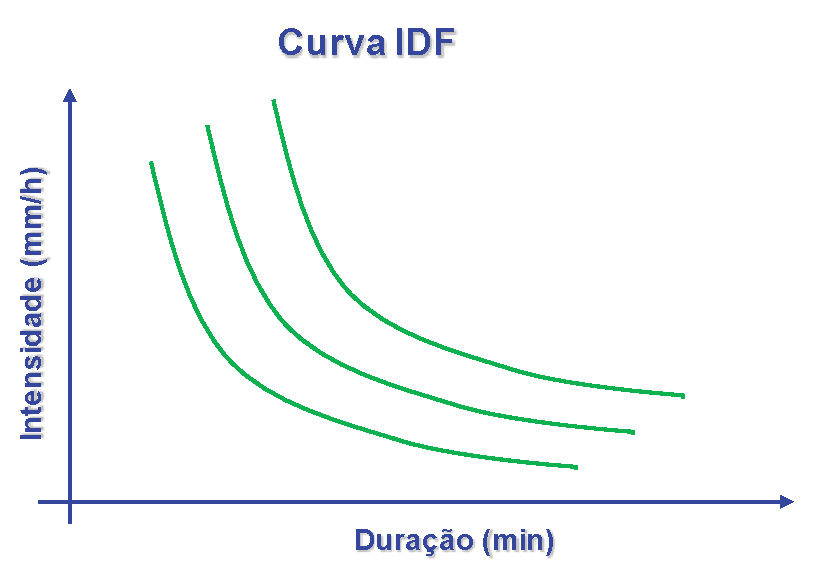
\includegraphics[width=0.8\textwidth]{Textuais/Figuras/curva-idf.pdf}
    \fonte{Autores}
    \label{fig:desagregacao}
\end{figure}